\documentclass[12pt,a4paper]{article}
%\usepackage{ctex}
\usepackage{amsmath,amscd,amsbsy,amssymb,latexsym,url,bm,amsthm}
\usepackage{epsfig,graphicx,subfigure}
\usepackage{enumitem,balance}
\usepackage{wrapfig}
\usepackage{mathrsfs,euscript}
\usepackage[x11names,svgnames,dvipsnames]{xcolor}
\usepackage{hyperref}
\usepackage[vlined,ruled,commentsnumbered,linesnumbered]{algorithm2e}
\usepackage{listings}
\usepackage{multicol}
%\usepackage{fontspec}

\renewcommand{\listalgorithmcfname}{List of Algorithms}
\renewcommand{\algorithmcfname}{Alg}

\newtheorem{theorem}{Theorem}
\newtheorem{lemma}[theorem]{Lemma}
\newtheorem{proposition}[theorem]{Proposition}
\newtheorem{corollary}[theorem]{Corollary}
\newtheorem{exercise}{Exercise}
\newtheorem*{solution}{Solution}
\newtheorem{definition}{Definition}
\theoremstyle{definition}


%\numberwithin{equation}{section}
%\numberwithin{figure}{section}

\renewcommand{\thefootnote}{\fnsymbol{footnote}}

\newcommand{\postscript}[2]
 {\setlength{\epsfxsize}{#2\hsize}
  \centerline{\epsfbox{#1}}}

\renewcommand{\baselinestretch}{1.0}

\setlength{\oddsidemargin}{-0.365in}
\setlength{\evensidemargin}{-0.365in}
\setlength{\topmargin}{-0.3in}
\setlength{\headheight}{0in}
\setlength{\headsep}{0in}
\setlength{\textheight}{10.1in}
\setlength{\textwidth}{7in}
\makeatletter \renewenvironment{proof}[1][Proof] {\par\pushQED{\qed}\normalfont\topsep6\p@\@plus6\p@\relax\trivlist\item[\hskip\labelsep\bfseries#1\@addpunct{.}]\ignorespaces}{\popQED\endtrivlist\@endpefalse} \makeatother
\makeatletter
\renewenvironment{solution}[1][Solution] {\par\pushQED{\qed}\normalfont\topsep6\p@\@plus6\p@\relax\trivlist\item[\hskip\labelsep\bfseries#1\@addpunct{.}]\ignorespaces}{\popQED\endtrivlist\@endpefalse} \makeatother


\definecolor{codegreen}{rgb}{0.44,0.68,0.28}
\definecolor{codegray}{rgb}{0.5,0.5,0.5}
\definecolor{codepurple}{rgb}{0.58,0,0.82}
\definecolor{backcolour}{rgb}{0.96,0.96,0.96}

\lstset{
language=C++,
frame=shadowbox,
keywordstyle = \color{blue}\bfseries,
commentstyle=\color{codegreen},
tabsize = 4,
backgroundcolor=\color{backcolour},
numbers=left,
numbersep=5pt,
breaklines=true,
emph = {int,float,double,char},emphstyle=\color{orange},
emph ={[2]const, typedef},emphstyle = {[2]\color{red}} }



\begin{document}
\noindent

%========================================================================
\noindent\framebox[\linewidth]{\shortstack[c]{
\Large{\textbf{Lab05-Priority Queues and Application}}\vspace{1mm}\\
VE281 - Data Structures and Algorithms, Xiaofeng Gao, Autumn 2019}}
%CS26019 - Algorithm Design and Analysis, Xiaofeng Gao, Autumn 2019}}
\begin{center}
\footnotesize{\color{blue}$*$ Name:Wu Jiayao  \quad Student ID:517370910257 \quad Email: jiayaowu1999@sjtu.edu.cn}
\end{center}
\section{Performance Comparison}
\subsection{Testing settings}
\begin{enumerate}
    \item For this report, 11 different width are used to compare the performance, listed as follows
    $$
    50,230,410,590,770,950,1130,1310,1490,1670,1850
    $$ 
    \item For each of the five size, 30 grids are generated then tested before getting an average running time for this size.
    \item The figure is plotted through Excel.
\end{enumerate}
\subsection{Performance of Unsorted Heap}
\begin{table}[h]
    \centering
    \begin{tabular}{|c|c|}
    \hline
    Size & Time for Unsorted(s) \\ \hline
    50   & 0.001    \\ \hline
    230  & 0.023    \\ \hline
    410  & 0.124    \\ \hline
    590  & 0.384    \\ \hline
    770  & 1.035    \\ \hline
    950  & 1.891    \\ \hline
    1130 & 2.927    \\ \hline
    1310 & 4.641    \\ \hline
    1490 & 7.268    \\ \hline
    1670 & 11.495   \\ \hline
    1850 & 17.518   \\ \hline
    \end{tabular}
    \caption{Running time of grids with 11 different size by Unsorted Heap}
    \label{unsorted}
\end{table}
\newpage
\subsection{Performance of Binary Heap}
\begin{table}[h]
    \centering
    \begin{tabular}{|c|c|}
    \hline
    Size & Time for Binary(s) \\ \hline
    50   & 0.000  \\ \hline
    230  & 0.010  \\ \hline
    410  & 0.024  \\ \hline
    590  & 0.069  \\ \hline
    770  & 0.127  \\ \hline
    950  & 0.178  \\ \hline
    1130 & 0.243  \\ \hline
    1310 & 0.327  \\ \hline
    1490 & 0.476  \\ \hline
    1670 & 0.654  \\ \hline
    1850 & 0.836  \\ \hline
    \end{tabular}
    \caption{Running time of grids with 11 different size by Binary Heap}
    \label{binary}
\end{table}
\subsection{Performance of Fibonacci Heap}
\begin{table}[h]
    \centering
    \begin{tabular}{|c|c|}
    \hline
    Size & Time for Fibonacci(s) \\ \hline
    50   & 0.001     \\ \hline
    230  & 0.031     \\ \hline
    410  & 0.121     \\ \hline
    590  & 0.283     \\ \hline
    770  & 0.583     \\ \hline
    950  & 1.073     \\ \hline
    1130 & 1.548     \\ \hline
    1310 & 2.389     \\ \hline
    1490 & 3.416     \\ \hline
    1670 & 4.920     \\ \hline
    1850 & 6.651     \\ \hline
    \end{tabular}
    \caption{Running time of grids with 11 different size by Fibonacci Heap}
    \label{fib}
\end{table}
\newpage
\subsection{Overall Comparison}
\begin{figure}[htbp]
    \centering
    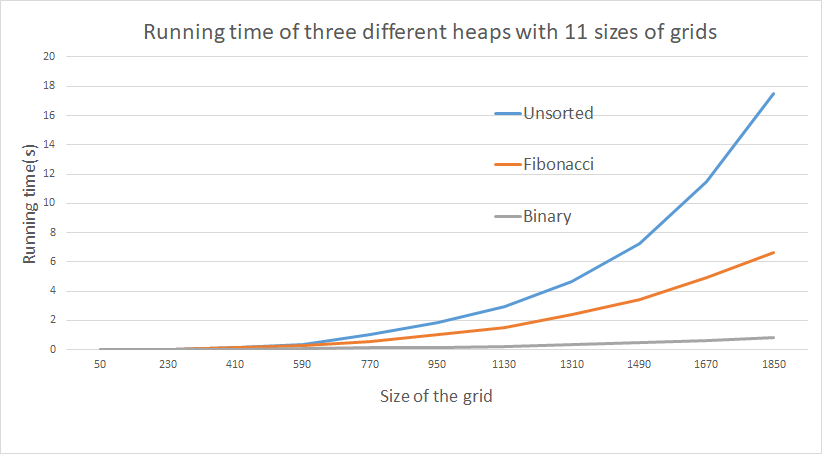
\includegraphics[width=0.7\textwidth]{three.png}
    \caption{Running time of grids with 11 different size}
\end{figure}
\section{Conclusion and Discussion}
\par In Conclusion, in grids with relatively large size, priority queue implemented with binary heap performs the best with the shortest average running time, followed by that by Fibonacci Heap, the last the unsorted heap.
\par Theoratically, Fibonacci heap should be of similar or less running time with/than binary heap, since they have the same theoratical time complexity for \textbf{dequeue\_min}, while \textbf{enqueue} operatrion is constant time for Fibonacci heaps but $\mathcal{O}(\log n)$ for binary heaps.
\begin{table}[h]
    \centering
    \begin{tabular}{|c|c|c|}
    \hline
    Type & enqueue & dequeue\_min \\ \hline
    Unsorted  & $\Theta(1)$ & $\Theta(n)$ \\ \hline
    Binary  & $\mathcal{O}(\log n)$ & $\mathcal{O}(\log n)$ \\ \hline
    Fibonacci  & $\Theta(1)$ & $\mathcal{O}(\log n)$ \\ \hline
    \end{tabular}
    \caption{Theoratical running time of two operations for different types of priority queues}
    \label{tab:my-table}
\end{table}
\par The reason that Fibonacci heap performs much worse than binary heap is that in this path searching algorithm, quite a large amount of \textbf{dequeue\_min} operations are needed to complete such computing. For Fibonacci heap, \textbf{dequeue\_min} takes a great effort since all its maintainence work is done during \textbf{dequeue\_min}.
\newpage
\section*{Appendix}
\subsection*{priority\_queue.h}
\begin{lstlisting}
#ifndef PRIORITY_QUEUE_H
#define PRIORITY_QUEUE_H

#include <functional>
#include <vector>

// OVERVIEW: A simple interface that implements a generic heap.
//           Runtime specifications assume constant time comparison and
//           copying. TYPE is the type of the elements stored in the priority
//           queue. COMP is a functor, which returns the comparison result of
//           two elements of the type TYPE. See test_heap.cpp for more details
//           on functor.
template<typename TYPE, typename COMP = std::less<TYPE> >
class priority_queue {
public:
    typedef unsigned size_type;

    virtual ~priority_queue() {}

    // EFFECTS: Add a new element to the heap.
    // MODIFIES: this
    // RUNTIME: O(n) - some implementations *must* have tighter bounds (see
    //          specialized headers).
    virtual void enqueue(const TYPE &val) = 0;

    // EFFECTS: Remove and return the smallest element from the heap.
    // REQUIRES: The heap is not empty.
    //           Note: We will not run tests on your code that would require it
    //           to dequeue an element when the heap is empty.
    // MODIFIES: this
    // RUNTIME: O(n) - some implementations *must* have tighter bounds (see
    //          specialized headers).
    virtual TYPE dequeue_min() = 0;

    // EFFECTS: Return the smallest element of the heap.
    // REQUIRES: The heap is not empty.
    // RUNTIME: O(n) - some implementations *must* have tighter bounds (see
    //          specialized headers).
    virtual const TYPE &get_min() const = 0;

    // EFFECTS: Get the number of elements in the heap.
    // RUNTIME: O(1)
    virtual size_type size() const = 0;

    // EFFECTS: Return true if the heap is empty.
    // RUNTIME: O(1)
    virtual bool empty() const = 0;

};

#endif //PRIORITY_QUEUE_H
    
\end{lstlisting}
\subsection*{binary\_heap.h}
\begin{lstlisting}
#ifndef BINARY_HEAP_H
#define BINARY_HEAP_H

#include "priority_queue.h"
#include <algorithm>

// OVERVIEW: A specialized version of the 'heap' ADT implemented as a binary
//           heap.
template <typename TYPE, typename COMP = std::less<TYPE>>
class binary_heap : public priority_queue<TYPE, COMP>
{
public:
    typedef unsigned size_type;

    // EFFECTS: Construct an empty heap with an optional comparison functor.
    //          See test_heap.cpp for more details on functor.
    // MODIFIES: this
    // RUNTIME: O(1)
    binary_heap(COMP comp = COMP());

    // EFFECTS: Add a new element to the heap.
    // MODIFIES: this
    // RUNTIME: O(log(n))
    virtual void enqueue(const TYPE &val);

    // EFFECTS: Remove and return the smallest element from the heap.
    // REQUIRES: The heap is not empty.
    // MODIFIES: this
    // RUNTIME: O(log(n))
    virtual TYPE dequeue_min();

    // EFFECTS: Return the smallest element of the heap.
    // REQUIRES: The heap is not empty.
    // RUNTIME: O(1)
    virtual const TYPE &get_min() const;

    // EFFECTS: Get the number of elements in the heap.
    // RUNTIME: O(1)
    virtual size_type size() const;

    // EFFECTS: Return true if the heap is empty.
    // RUNTIME: O(1)
    virtual bool empty() const;

private:
    // Note: This vector *must* be used in your heap implementation.
    std::vector<TYPE> data;
    // Note: compare is a functor object
    COMP compare;

private:
    virtual void percolate_up(int id);
    virtual void percolate_down(int id);

private:
    // Add any additional member functions or data you require here.
};

template <typename TYPE, typename COMP>
binary_heap<TYPE, COMP>::binary_heap(COMP comp)
{
    compare = comp;
    // Fill in the remaining lines if you need.
}

template <typename TYPE, typename COMP>
void binary_heap<TYPE, COMP>::enqueue(const TYPE &val)
{
    data.push_back(val);
    percolate_up(int(size())-1);
}

template <typename TYPE, typename COMP>
TYPE binary_heap<TYPE, COMP>::dequeue_min()
{
    TYPE res = data.front();
    data[0] = data.back();
    data.pop_back();
    if (!empty())
    {
        percolate_down(0);
    }
    return res;
}

template <typename TYPE, typename COMP>
const TYPE &binary_heap<TYPE, COMP>::get_min() const
{
    return data.front();
}

template <typename TYPE, typename COMP>
bool binary_heap<TYPE, COMP>::empty() const
{
    return data.empty();
}

template <typename TYPE, typename COMP>
unsigned binary_heap<TYPE, COMP>::size() const
{
    return data.size();
}

template <typename TYPE, typename COMP>
void binary_heap<TYPE, COMP>::percolate_up(int id)
{
    while (id > 0 && compare(data[id],data[(id-1) / 2]))
    {
        TYPE tmp = data[(id-1) / 2];
        data[(id-1) / 2] = data[id];
        data[id] = tmp;
        id = (id-1) / 2;
    }
}

template <typename TYPE, typename COMP>
void binary_heap<TYPE, COMP>::percolate_down(int id)
{
    for (int j = id*2 + 1; j < size(); j = id*2+1)
    {
        if (j < int(size())-1 && compare(data[j+1],data[j]))
        {
            j++;
        }
        if (compare(data[id],data[j]))
        {
            break;
        }
        TYPE tmp = data[id];
        data[id] = data[j];
        data[j] = tmp;
        id = j;
    }
}
#endif //BINARY_HEAP_H
\end{lstlisting}
\subsection*{unsorted\_heap.h}
\begin{lstlisting}
#ifndef UNSORTED_HEAP_H
#define UNSORTED_HEAP_H

#include "priority_queue.h"
#include <algorithm>

// OVERVIEW: A specialized version of the 'heap' ADT that is implemented with
//           an underlying unordered array-based container. Every time a min
//           is required, a linear search is performed.
template <typename TYPE, typename COMP = std::less<TYPE>>
class unsorted_heap : public priority_queue<TYPE, COMP>
{
public:
    typedef unsigned size_type;

    // EFFECTS: Construct an empty heap with an optional comparison functor.
    //          See test_heap.cpp for more details on functor.
    // MODIFIES: this
    // RUNTIME: O(1)
    unsorted_heap(COMP comp = COMP());

    // EFFECTS: Add a new element to the heap.
    // MODIFIES: this
    // RUNTIME: O(1)
    virtual void enqueue(const TYPE &val);

    // EFFECTS: Remove and return the smallest element from the heap.
    // REQUIRES: The heap is not empty.
    // MODIFIES: this
    // RUNTIME: O(n)
    virtual TYPE dequeue_min();

    // EFFECTS: Return the smallest element of the heap.
    // REQUIRES: The heap is not empty.
    // RUNTIME: O(n)
    virtual const TYPE &get_min() const;

    // EFFECTS: Get the number of elements in the heap.
    // RUNTIME: O(1)
    virtual size_type size() const;

    // EFFECTS: Return true if the heap is empty.
    // RUNTIME: O(1)
    virtual bool empty() const;

private:
    // Note: This vector *must* be used in your heap implementation.
    std::vector<TYPE> data;
    // Note: compare is a functor object
    COMP compare;

private:
    // Add any additional member functions or data you require here.
};

template <typename TYPE, typename COMP>
unsorted_heap<TYPE, COMP>::unsorted_heap(COMP comp)
{
    compare = comp;
    // Fill in the remaining lines if you need.
}

template <typename TYPE, typename COMP>
void unsorted_heap<TYPE, COMP>::enqueue(const TYPE &val)
{
    data.push_back(val);
}

template <typename TYPE, typename COMP>
TYPE unsorted_heap<TYPE, COMP>::dequeue_min()
{
    auto min = data.begin();
    for (auto it = data.begin(); it != data.end();it++)
    {
        if(compare((*it),(*min)))
        {
            min = it;
        }
    }
    TYPE res = *min;
    *min = data.back();
    data.pop_back();
    return res;
}

template <typename TYPE, typename COMP>
const TYPE &unsorted_heap<TYPE, COMP>::get_min() const
{
    return data[0];
}

template <typename TYPE, typename COMP>
bool unsorted_heap<TYPE, COMP>::empty() const
{
    return data.empty();
}

template <typename TYPE, typename COMP>
unsigned unsorted_heap<TYPE, COMP>::size() const
{
    return data.size();
}

#endif //UNSORTED_HEAP_H
     
\end{lstlisting}
\subsection*{fib\_heap.h}
\begin{lstlisting}
#ifndef FIB_HEAP_H
#define FIB_HEAP_H

#include "priority_queue.h"
#include <algorithm>
#include <cmath>

// OVERVIEW: A specialized version of the 'heap' ADT implemented as a
//           Fibonacci heap.
template <typename TYPE, typename COMP = std::less<TYPE>>
class fib_heap : public priority_queue<TYPE, COMP>
{
public:
    typedef unsigned size_type;

    // EFFECTS: Construct an empty heap with an optional comparison functor.
    //          See test_heap.cpp for more details on functor.
    // MODIFIES: this
    // RUNTIME: O(1)
    fib_heap(COMP comp = COMP()):compare(comp),heapSize(0),min(NULL){};

    // EFFECTS: Deconstruct the heap with no memory leak.
    // MODIFIES: this
    // RUNTIME: O(n)
    ~fib_heap();

    // EFFECTS: Add a new element to the heap.
    // MODIFIES: this
    // RUNTIME: O(1)
    virtual void enqueue(const TYPE &val);

    // EFFECTS: Remove and return the smallest element from the heap.
    // REQUIRES: The heap is not empty.
    // MODIFIES: this
    // RUNTIME: Amortized O(log(n))
    virtual TYPE dequeue_min();

    // EFFECTS: Return the smallest element of the heap.
    // REQUIRES: The heap is not empty.
    // RUNTIME: O(1)
    virtual const TYPE &get_min() const;

    // EFFECTS: Get the number of elements in the heap.
    // RUNTIME: O(1)
    virtual size_type size() const;

    // EFFECTS: Return true if the heap is empty.
    // RUNTIME: O(1)
    virtual bool empty() const;

private:
    // Note: compare is a functor object
    COMP compare;

private:
    // Add any additional member functions or data you require here.
    // You may want to define a strcut/class to represent nodes in the heap and a
    // pointer to the min node in the heap.
    struct Node
    {
        TYPE val;
        Node *left;
        Node *right;
        Node *parent;
        Node *child;
        int degree;
        Node(const TYPE &_val) : val(_val)
        {
            left = right = this;
            child = parent = NULL;
            degree = 0;
        }
    };
    size_type heapSize;
    Node *min;
    
    void consolidate();

    void link(Node *y, Node *x);

    void clear(Node* x);
};

// Add the definitions of the member functions here. Please refer to
// binary_heap.h for the syntax.
template <typename TYPE, typename COMP>
fib_heap<TYPE, COMP>::~fib_heap()
{
//	while (!empty())
//	{
//		dequeue_min();
//	}
    clear(min);
}

template <typename TYPE, typename COMP>
void fib_heap<TYPE, COMP>::enqueue(const TYPE &val)
{
    Node *node = new Node(val);
    if (min == NULL)
    {
        min = node;
    }
    else
    {
        node->left = min;
        node->right = min->right;
        min->right->left = node;
        min->right = node;
        if (compare(val, min->val))
        {
            min = node;
        }
    }
    heapSize++;
}

template <typename TYPE, typename COMP>
TYPE fib_heap<TYPE, COMP>::dequeue_min()
{
    Node *z = min;
    TYPE res = z->val;
    while (z->child != NULL)
    {
        Node *p = z->child;
        p->parent = NULL;
        if (p == p->right)
        {
            z->child = NULL;
        }
        else
        {
            p->left->right = p->right;
            p->right->left = p->left;
            z->child = p->right;
        }
        p->right = min->right;
        p->left = min;
        min->right->left = p;
        min->right = p;
    }
    heapSize--;
    if (heapSize == 0)
    {
        min = NULL;
    }
    else
    {
        min = z->right;
        z->left->right = z->right;
        z->right->left = z->left;
        consolidate();
    }
    delete z;
    return res;
}

template<typename TYPE,typename COMP>
const TYPE &fib_heap<TYPE,COMP>::get_min() const
{
    return min->val;
}

template<typename TYPE,typename COMP>
unsigned int fib_heap<TYPE,COMP>::size() const
{
    return heapSize;
}

template<typename TYPE,typename COMP>
bool fib_heap<TYPE,COMP>::empty() const
{
    return heapSize==0;
}

template <typename TYPE, typename COMP>
void fib_heap<TYPE, COMP>::link(Node *y, Node *x)
{
    if (x->child == NULL)
    {
        y->left = y->right = y;
        y->parent = x;
        x->child = y;
    }
    else
    {
        y->left = x->child;
        y->right = x->child->right;
        x->child->right->left = y;
        x->child->right = y;
        y->parent = x;
    }
    x->degree++;
}

template <typename TYPE, typename COMP>
void fib_heap<TYPE, COMP>::consolidate()
{
    using namespace std;
    //int tmp_size = int(log(heapSize) / log((1 + sqrt(5)) / 2));
    int tmp_size = int(size());
    vector<Node *> array(tmp_size, NULL);
    Node *itr = min;
    while (1)
    {
        Node *x = itr;
        itr = itr->right;
        int d = x->degree;
        while (array[d] != NULL)
        {
            Node *y = array[d];
            if (compare(y->val,x->val))
            {
                Node *tmp = x;
                x = y;
                y = tmp;
            }
            link(y, x);
            array[d] = NULL;
            d++;
        }
        array[d] = x;
        if (itr == min)
        {
            break;
        }
    }
    min = NULL;
    for (auto &p : array)
    {
        if (p != NULL)
        {
            if (min == NULL)
            {
                min = p;
                p->left = p->right = p;
            }
            else
            {
                p->left = min;
                p->right = min->right;
                min->right->left = p;
                min->right = p;
                if (compare(p->val, min->val))
                {
                    min = p;
                }
            }
        }
    }
}

template <typename TYPE, typename COMP>
void fib_heap<TYPE, COMP>::clear(Node* x)
{
    if(x == NULL)
    {
        return;
    }
    Node* p = x;

    while(true)
    {
        Node* q = p->right;
        clear(p->child);
        delete p;
        p = q;
        if(p == x)
        {
            break;
        }
    }
}


#endif //FIB_HEAP_H
    
\end{lstlisting}
\subsection*{graph.h}
\begin{lstlisting}
#ifndef VE281LAB5_GRAPH_H
#define VE281LAB5_GRAPH_H
#include <vector>
#include "priority_queue.h"
#include "binary_heap.h"
#include "fib_heap.h"
#include "unsorted_heap.h"
#define FIB 1
#define BINARY 2
#define UNSORT 3
//#define TIME

struct myOption
{
    bool verbose;
    int implement;
};

struct Axis
{
    int r;
    int c;
};
class Vertex
{
public:
    int cost;
    int pathCost;
    int row;
    int column;
    bool visited;
    Axis prev;
    Vertex(int _row, int _column, int _cost):row(_row),column(_column),cost(_cost)
    {
        pathCost = 0;
        prev = {-1,-1};
        visited = false;
    }
    struct compare_t
    {
        bool operator()(Vertex *a,Vertex *b) const
        {
            if (a->pathCost < b->pathCost)
            {
                return true;
            }
            else if (a->pathCost == b->pathCost)
            {
                if(a->column < b->column)
                {
                    return true;
                }
                else if(a->column == b->column)
                {
                    if(a->row < b->row)
                    {
                        return true;
                    }
                }
            }
            return false;
        }
    };

};

class Graph
{
private:
    std::vector<std::vector<Vertex>> points;
    Axis start;
    Axis end;
    int shortest;
    int mode;
    int row_num;
    int column_num;
    bool verbose;
    priority_queue<Vertex*,Vertex::compare_t> *pq;
public:
    Graph(const myOption &option);
    ~Graph();
    void solve();
private:
    void check();
    Vertex& get_point(const Axis &a);
    int set_neighbor(Vertex* v, const int& a, const int &b);
    void track_path(const Axis &a);
    void result_print();
};

#endif //VE281LAB5_GRAPH_H

\end{lstlisting}
\subsection*{graph.cpp}
\begin{lstlisting}
#include "graph.h"
#include <iostream>
std::ostream &operator<<(std::ostream &os, const Axis &axis)
{
    return os << "(" << axis.c << ", " << axis.r << ")";
}

std::ostream &operator<<(std::ostream &os, const Vertex &v)
{
    return os << "(" << v.column << ", " << v.row << ")" << " with accumulated length " << v.pathCost ;
}

Graph::Graph(const myOption &option){
    using namespace std;
    cin >> column_num;
    cin >> row_num;
    int st_r = 0, st_c = 0;
    cin >> st_r;
    cin >> st_c;
    int ed_r = 0, ed_c = 0;
    cin >> ed_r;
    cin >> ed_c;
    for(int i = 0 ; i < row_num;i++)
    {
        points.emplace_back();
        for(int j = 0 ; j < column_num;j++)
        {
            int tmp = 0;
            cin >> tmp;
            points[i].emplace_back(i,j,tmp);
        }
    }
    start = {st_c,st_r};
    end = {ed_c,ed_r};
    shortest = 0;
    switch (option.implement)
    {
        case BINARY:
        {
            pq = new binary_heap<Vertex*,Vertex::compare_t>;
            break;
        }
        case UNSORT:
        {
            pq = new unsorted_heap<Vertex*,Vertex::compare_t>;
            break;
        }
        case FIB:
        {
            pq = new fib_heap<Vertex*,Vertex::compare_t>;
            break;
        }
        default:break;
    }
    verbose = option.verbose;
#ifdef TIME
    cout << row_num << ",";
#endif
    //check();
}

Graph::~Graph()
{
    delete pq;
}

void Graph::solve()
{
    using namespace std;
    int counter = 0;
    Vertex &s = get_point(start);
    s.pathCost = s.cost;
    s.visited = true;
    pq->enqueue(&s);
    std::string output;
    stringstream ss;
    while (!pq->empty())
    {
        if(verbose)
        {
            ss << "Step " << counter++ << "\n";
        }
        Vertex* minimum = pq->dequeue_min();
        if(verbose)
        {
            ss << "Choose cell " << *minimum << ".\n";
        }
        if(set_neighbor(minimum,0,1,ss) == 1)
            break;
        if(set_neighbor(minimum,1,0,ss) == 1)
            break;
        if(set_neighbor(minimum,0,-1,ss) == 1)
            break;
        if(set_neighbor(minimum,-1,0,ss) == 1)
            break;
        //std::cerr << "??" << "\n";
    }
#ifndef TIME
    result_print(ss);
    output = ss.str();
    cout << output;
#endif
}

void Graph::check()
{
    for(auto &p:points)
    {
        for(auto &q : p)
        {
            std::cout << q.cost << " ";
        }
        std::cout << std::endl;
    }
}

Vertex& Graph::get_point(const Axis &a)
{
    return points[a.r][a.c];
}

void Graph::result_print(std::stringstream &ss)
{
    ss << "The shortest path from "
            << start << " to " << end
            << " is " << shortest << ".\n"
            << "Path:" << "\n";
    track_path(end,ss);
}

void Graph::track_path(const Axis &a, std::stringstream &ss)
{
    Vertex &v = get_point(a);
    if(v.prev.r >= 0)
    {
        track_path(v.prev, ss);
    }
    ss << a << "\n";
}

int Graph::set_neighbor(Vertex* v, const int& r, const int &c,std::stringstream &ss)
{
    if(v->row + r >= 0 && v->row + r < row_num &&
        v->column + c >= 0 && v->column + c < column_num)
    {
        Vertex &neighbor = points[v->row+r][v->column+c];
        if(!neighbor.visited)
        {
            neighbor.visited = true;
            neighbor.pathCost = neighbor.cost + v->pathCost;
            neighbor.prev = {v->row,v->column};
            if(v->row+r == end.r && v->column + c == end.c)
            {
                if(verbose)
                    ss << "Cell " << neighbor << " is the ending point.\n";
                shortest = neighbor.pathCost;
                return 1;
            }
            else
            {
                pq->enqueue(&neighbor);
                if(verbose)
                    ss << "Cell " << neighbor << " is added into the queue.\n";
            }
        }

    }
    return 0;

}
    
    
\end{lstlisting}
\subsection*{interface.h}
\begin{lstlisting}
#ifndef VE281LAB5_INTERFACE_H
#define VE281LAB5_INTERFACE_H

#include "priority_queue.h"
#include "unsorted_heap.h"
#include "fib_heap.h"
#include "binary_heap.h"
#include "graph.h"

myOption parseArgs(int argc, char** argv);

#endif //VE281LAB5_INTERFACE_H

\end{lstlisting}
\subsection*{interface.cpp}
\begin{lstlisting}
#include "interface.h"
#include <cstdlib>
#include <cstdio>
#include <cstring>
#include <unistd.h>
#include <getopt.h>
#include <iostream>
//#define  DEBUG
myOption parseArgs(int argc, char** argv)
{
    using namespace std;
    int inputChar = 0;
    struct option opts[] = {
            {"implementation", 1, NULL, 'i'},
            {"verbose", 0, NULL, 'v'}
    };
    myOption res;
    res.verbose = false;
    res.implement = -1;
    while((inputChar = getopt_long(argc,argv,"i:v",opts,NULL)) != -1)
    {
        switch(inputChar)
        {
            case 'i':
            {
#ifdef DEBUG
                cout << optarg << endl;
#endif
                if(!strcmp(optarg,"BINARY"))
                {
                    res.implement = BINARY;
                }
                else if(!strcmp(optarg,"UNSORTED"))
                {
                    res.implement = UNSORT;
                }
                else if(!strcmp(optarg,"FIBONACCI"))
                {
                    res.implement = FIB;
                }
                break;
            }
            case 'v':
            {
                res.verbose = true;
                break;
            }
        }
    }
    return res;
}

\end{lstlisting}
\subsection*{main.cpp}
\begin{lstlisting}
#include "interface.h"
#include "graph.h"
#include <iostream>
#include<time.h>
int main(int argc,char** argv)
{
    using namespace std;
    ios::sync_with_stdio(false);
    cin.tie(0);
    myOption option = parseArgs(argc,argv);
    Graph graph(option);
    clock_t start = clock();
    graph.solve();
#ifdef TIME
    cout << float(clock() - start)/CLOCKS_PER_SEC << "\n";
#else
    cerr << "Time: " << float(clock() - start)/CLOCKS_PER_SEC << "\n";
#endif
}
\end{lstlisting}
\end{document}